
\documentclass{article} % For LaTeX2e
\usepackage{iclr2022_conference,times}

% Optional math commands from https://github.com/goodfeli/dlbook_notation.
\input{math_commands.tex}
\newcommand{\real}[1]{\mathbb{R}^{#1}}

\newcommand{\imageDataset}{\mathcal{X}}
\newcommand{\image}{\vx}

\newcommand{\latentDataset}{\mathcal{L}}
\newcommand{\latent}{\vz}

\newcommand{\vqganEncoder}{E}
\newcommand{\vqganDecoder}{G}
\newcommand{\vqganCodebook}{\mathcal{C}}
\newcommand{\vqganDownsample}{f}
\newcommand{\codebookVector}{\ve}


\usepackage[pagebackref,breaklinks,colorlinks]{hyperref}
\usepackage{url}

\usepackage[margin=1in]{geometry}
\usepackage{graphicx}
\usepackage{amsmath}
\usepackage{amssymb}
\usepackage{booktabs}
\usepackage{overpic}

\usepackage[capitalize]{cleveref}
\crefname{section}{Sec.}{Secs.}
\Crefname{section}{Section}{Sections}
\Crefname{table}{Table}{Tables}
\crefname{table}{Tab.}{Tabs.}

\title{Megapixel Image Generation with Step-unrolled Denoising Autoencoders}

% Authors must not appear in the submitted version. They should be hidden
% as long as the \iclrfinalcopy macro remains commented out below.
% Non-anonymous submissions will be rejected without review.

\author{Alex F. McKinney \& Chris G. Willcocks \\
Department of Computer Science\\
Durham University\\
Durham, UK \\
\texttt{\{alexander.f.mckinney,christopher.g.willcocks\}@durham.ac.uk} \\
}

% The \author macro works with any number of authors. There are two commands
% used to separate the names and addresses of multiple authors: \And and \AND.
%
% Using \And between authors leaves it to \LaTeX{} to determine where to break
% the lines. Using \AND forces a linebreak at that point. So, if \LaTeX{}
% puts 3 of 4 authors names on the first line, and the last on the second
% line, try using \AND instead of \And before the third author name.

\newcommand{\fix}{\marginpar{FIX}}
\newcommand{\new}{\marginpar{NEW}}

\iclrfinalcopy % Uncomment for camera-ready version, but NOT for submission.
\begin{document}

\maketitle

\begin{abstract}
    Advancements in deep generative modelling has pushed sample resolution higher
whilst reducing computational requirements and sampling speeds. One approach
works in two stages: training a powerful vector-quantization image model and
then training a second discrete prior to predict discrete tokens corresponding
to image patches. Early work produced high fidelity and diverse samples, but
were prohibitively slow to sample from as they were autoregressive in nature.
Later work exploited discrete diffusion models in order to allow for parallel
token prediction, dramatically speeding up the sampling process. In this work,
we push the sampling speed and computational requirements further by replacing
discrete diffusion models with denoising autoencoders, as well as modifications
to the Transformer backbone including axial embeddings, an hourglass structure,
and resampling layers more suited to image tasks. Furthermore, the
non-autoregressive nature of the model allows for arbitrary inpainting patterns.
Finally, we train new vector-quantization models to allow for the sampling of
upwards of a megapixel images in seconds, and without relying on sliding window
mechanisms.

% Reference FYI from our recent submission that's similar to you (it's not the best abstract, a bit too wordy, but not too bad):
% Whilst diffusion probabilistic models can generate high quality image content, key limitations remain in terms of both generating high-resolution imagery and their associated high computational requirements. Recent Vector-Quantized image models have overcome this limitation of image resolution but are prohibitively slow and unidirectional as they generate tokens via element-wise autoregressive sampling from the prior. By contrast, in this paper we propose a novel discrete diffusion probabilistic model prior which enables parallel prediction of Vector-Quantized tokens by using an unconstrained Transformer architecture as the backbone. During training, tokens are randomly masked in an order-agnostic manner and the Transformer learns to predict the original tokens. This parallelism of Vector-Quantized token prediction in turn facilitates unconditional generation of globally consistent high-resolution and diverse imagery at a fraction of the computational expense. In this manner, we can generate image resolutions exceeding that of the original training set samples whilst additionally provisioning per-image likelihood estimates (in a departure from generative adversarial approaches). Our approach achieves state-of-the-art results in terms of Density (LSUN Bedroom: 1.51; LSUN Churches: 1.12; FFHQ: 1.20) and Coverage (LSUN Bedroom: 0.83; LSUN Churches: 0.73; FFHQ: 0.80), and performs competitively on FID (LSUN Bedroom: 3.64; LSUN Churches: 4.07; FFHQ: 6.11) whilst offering advantages in terms of both computation and reduced training set requirements.
\end{abstract}

\begin{figure}[ht]
    \centering
    \includegraphics[width=1.0\linewidth]{figures/sample1024.png}
    \caption{
        High-resolution samples produced using our non-autoregressive approach.
        Each $1024 \times 1024$ sample was generated in $\approx 2$ seconds on a
        GTX 1080Ti -- including both discrete latent sampling and subsequent
        decoding. The SUNDAE sampler was trained in 4 days on a single V100
        32GB.
    }
\end{figure}

\section{Introduction}\label{sec:intro}
An ideal deep generative model would satisfy three key requirements:
high-quality samples, sample diversity via mode coverage, and computational
inexpensive sampling. Arguably, there are other desirable properties such as a
meaningful latent space and exact likelihood calculation, however no current
generative model can satisfy all three requirements -- let alone additional
attractive properties -- thus forming the so-called generative modelling
trilemma~\cite{xiao2021trilemma}.

Models such as \glspl{gan}~\cite{goodfellow2014gan}
excel at high-quality and fast sampling, but often fail to model the entire data
distribution due to not directly optimising for likelihood -- using an
adversarial loss as a proxy. \Glspl{vae}~\cite{kingma2013vae} offer
excellent mode coverage and fast sampling speeds, but the resulting samples are
often blurry even at small resolutions, and have little hope of scaling to
greater resolutions like \glspl{gan}.

\Gls{ar} models such as PixelSnail~\cite{chen2017snail}, Image
Transformer~\cite{parmar2018image}, and DALL-E~\cite{parmar2018image} have
demonstrated respectable sample quality and mode coverage, even including
zero-shot image generation~\cite{ramesh2021dalle}. However, they are
computationally expensive to sample from, requiring many network iterations,
making them infeasible for interactive applications. \Glspl{ddpm}~\cite{ho2020ddpm}
and \glspl{sbm}~\cite{song2019sbm,song2020sde,song2021mlt} produce
samples that rival or even exceed the quality of \glspl{gan}~\cite{dhariwal2021ddpm}
whilst still providing good mode coverage, but are still plagued by potentially
requiring thousands of network evaluations.

Vector-quantized image
modelling~\cite{oord2017vqvae,razavi2019generating,esser2021taming} alleviates
sampling speed issues in \gls{ar} methods by reducing the spatial dimension at
which \gls{ar} sampling occurs. This results in excellent quality samples whilst
improving sampling speeds, but often requires a two-stage approach and still
does not match the speed of \glspl{gan}. Recent work has applied \gls{vq}
methods to diffusion models~\cite{bondtaylor2021unleashing} allowing for fast
parallel decoding. Other work does not use vector-quantized spaces, but latent
spaces nonetheless, to accelerate
sampling~\cite{xiao2021trilemma,vahdat2021sbmlatent}.

From this brief overview of generative modelling literature, it is clear that
indeed no single model satisfies all three conditions. This therefore motivates
research into explicitly addressing this trilemma. In this work, we move towards
such a solution, beginning from existing work applying generative models to
discrete latents. This provides an excellent starting point in terms of sample
quality and a respectable amount of mode coverage, but an unacceptably slow
sampling speed despite the reduced spatial dimension of the discrete latent
space. We directly address this issue by instead sampling discrete latents using
modern \gls{nar} generative models in an effort to close the gap, sampling speed
wise, with constant iteration complexity models such as \glspl{gan}.
Specifically, we use discrete \gls{sundae}~\cite{savinov2022stepunrolled} to
gradually denoise samples from a uniform prior into one that matches the prior
over the discrete latent space defined by a pre-trained \gls{vqgan} model. This
forms our first research question, whether \gls{sundae} models is suitable
paradigm for sampling discrete latent codes. As a result of our studies, we find
that indeed they are highly suited for this task.

These discrete \gls{sundae} models have only previously be applied to
language modelling tasks~\cite{savinov2022stepunrolled}. In their work, they
used transformer~\cite{vaswani2017attention} architectures to form their
autoencoder. In parallel, a noticeably more efficient variant of transformers --
the Hourglass Transformer~\cite{nawrot2021hierarchical} -- was released, which
has a hierarchical architecture aimed at language and image modelling tasks,
though potentially flawed on the latter. This raises a second research question,
whether the approach introduced in~\citet{savinov2022stepunrolled} is also
suited for latent modelling, and whether the hierarchical approach introduced
in~\citet{nawrot2021hierarchical} can be further improved upon. As a result of
our studies, we find that although they are suited for latent modelling, there
are many modifications we can make to improve their performance further.

Given a fast sampling and an efficient transformer architecture, we are
potentially left with a highly scaleable (with respect to spatial resolution)
model. This raises a third and final research question, whether our new approach
allows for the generation of extremely high resolution images in a time frame
that would permit fully- or near-interactive use. Again, as a result of our
studies, we find that this is indeed the case, proven by the synthesis of $1024
\times 1024$ images in as few as 2 seconds on a consumer-grade GPU. To our
knowledge, this is the fastest sampling model at this resolution, with the
exception of pure \gls{gan}-based approaches. This required the training of our
own \gls{vqgan} model, which was, also to our knowledge, the largest \gls{vqgan} model
trained in terms of input size.

%In this work, we aim to move towards satisfying all three key requirements for
%an ideal generative model. Like previous work, we use a vector-quantized image
%model to reduce the spatial dimension of the signal we wish to sample. We then
%apply new language models to instead model the distribution of discrete latents,
%ultimately obtaining a powerful prior over the discrete latents. With this and a
%discrete latent decoder, we obtain the final generative model, allowing sampling
%of images in a very low number of steps. We go further, and train our own
%VQ-GAN~\cite{esser2021taming} at resolutions higher than ever trained before to
%our knowledge, ultimately allowing for the sampling of $1024 \times 1024$ RGB
%images in only two seconds on a consumer-grade GPU.

Our project objectives were as follows:
\begin{itemize}
    \item Apply \gls{sundae} to the task of \acrshort{vq} latent generation and
        ultimately image generation, and perform analysis into their advantages
        of being used for this task over existing approaches, including both
        \gls{ar} and \gls{nar} solutions.

    \item Analyse the methods used in \citet{savinov2022stepunrolled} and
        \citet{nawrot2021hierarchical} and design modifications that make these
        approaches more suitable for \acrshort{vq} latent modelling.

    \item Attempt to scale our model to extremely high resolution images and
        analyse successes and failures when operating at such resolutions. 

\end{itemize}


\section{Related Work}\label{sec:related}
% TODO: lacks some narrative flow between sections

% TODO: end would benefit from "summary section" (not sure what that means) that
% reflects on high level trends in the literature, building into a proposed
% strategy and thus flowing into the methodology.
This work builds upon much prior research into powerful deep generative
models, self-supervised methods, and efficient
transformer architectures. We briefly cover relevant prior work into deep
generative models in general in \S\ref{subsec:agm}-\ref{subsec:vqmodelling}, a
particular \acrshort{nar} generative model we wish to build upon in
\S\ref{subsec:sundae}, and a recent and highly effective development into a
efficient transformer architecture in \S\ref{subsec:hourglass}. For a full
review on generative modelling we direct the reader to
\citet{bondtaylor2021review}, and for further details on \gls{sundae} and
hourglass transformers we direct the reader to \citet{savinov2022stepunrolled}
and \citet{nawrot2021hierarchical} respectively.

\begin{figure}
    \centering
    \includesvg[width=\textwidth]{figures/AR-NAR.svg}
    \caption{
        \textbf{Left:} Visualization of \acrfull{ar} sampling. \gls{ar} sampling
        proceeds one item at a time, resulting in the number of sampling steps
        being equal to the dimensionality of the input. For each prediction, a
        probability distribution over possible tokens is predicted and then
        sampled from. Each prediction can only make use of past context --
        indicated as a green position -- so not to violate the autoregressive
        property.
        \textbf{Right:} Visualization of \acrfull{nar} sampling. \gls{nar}
        sampling can sample an arbitrary number of items in parallel, including
        ones previously sampled, allowing for self-correction. It can freely use
        all context available to it, allowing for flexible inpainting and
        potentially better predictions.
    }
\end{figure}

\subsection{Autoregressive Generative Models}
\label{subsec:agm}
One major deep generative model family is \acrfull{ar} models, characterised by
a training and inference process based on the probabilistic chain rule. During
training, they directly aim to maximise the likelihood of the data they are
trained on, which leads to excellent mode coverage. Prior work using these
methods resulted in impressive results in terms of both sample quality and
diversity, but are ultimately unwieldy for use in real world applications due to
their slow sampling speed.

The slow sampling speed is due to their sequential nature, defined by the chain
rule of probability. Given an input $\image = \{ \pixel{1}, \pixel{2}, \dots,
\pixel{n} \}$, an \gls{ar} model $p_\theta(\cdot)$ can generates new
samples sequentially:
\begin{equation}\label{eq:ar}
    p_\theta(\image) = p_\theta(\pixel{1}, \dots, \pixel{n}) =
    \prod\limits^{n}_{i=1} p_\theta(\pixel{i} \vert \pixel{1}, \dots, \pixel{i-1})
\end{equation}
meaning that the number of sampling steps is equal to the size of the
decomposition of $\image$, making this slow for large inputs.

For certain tasks, the ordering of the decomposition of $\image$ is obvious, for
example on text or speech. For images this is less obvious, however typically a
raster scan ordering is used. Certain \gls{ar} models are order-agnostic,
allow for arbitrary ordering to be used during training and inference.

One class of \gls{ar} models are \glspl{rnn} which are an early example of using
neural networks to model sequential data, such as text, audio, time-series data,
or even vector handwriting strokes. Though they can be used as purely
classification or regression models, they are also suited for use as generative
models by modelling the relationship shown in Equation~\ref{eq:ar}. They do
suffer from a number of issues, most notably vanishing
gradients~\cite{pascanu2012rnn} and inability to model long-range relationships
between items in the input. \Glspl{lstm}~\cite{hoch1997lstm} improved upon them
further by introducing dedicated memory units, allowing for the modelling of
longer range relationships. Later \glspl{gru}~\cite{cho2014gru} simplified the
architecture whilst still retaining good performance. With the advent of
transformer architectures~\cite{vaswani2017attention}, modelling even longer
relationships became possible, even at a full-document level. It also intro cued
the capability to train on all sequence elements in parallel through the use of
causal masking, therefore not violating the autoregressive property.

Applying \gls{ar} models to images followed a similar trend.
PixelRNN~\cite{oord2016pixelrnn} used two-dimensional recurrent layers and
residual connections to model the distribution of raw pixel values. The same
paper also introduced PixelCNN, which it claims had worse performance but were
faster to train. These were extended to allow for conditional generation
in~\cite{oord2016pixelcnn}. Later work augmented PixelCNN with self-attention
mechanism, forming PixelSnail~\cite{chen2017snail}, which can therefore model
longer relationships than a fully convolutional or recurrent architecture. Image
Transformer~\cite{parmar2018image} later applied transformer architectures to
the same task through an effective but altogether conceptually simple approach.

\subsection{Non-autoregressive Generative Models}
\label{subsec:nagm}
\Acrfull{nar} generative models include \glspl{gan}, \glspl{sbm} and
\glspl{ddpm}, flow-based models, \glspl{ebm}, and implicit models. Though the
number of sampling steps is now independent of the data dimensionality (as we no
longer use the chain rule of probability to sample) the actual number of steps
varies greatly: from single-step generation in \glspl{gan} to potentially many
thousands in the original diffusion model literature.

% TODO: discuss briefly each from of NAR model and its strengths/weaknesses
% - [X] GAN
% - [X] Variational autoencoders
% - [X] SBM / DDPM
% - [X] Normalizing flows

Perhaps the most infamous class of \gls{nar} generative model -- or perhaps
generative model overall -- are \acrfullpl{gan}~\cite{goodfellow2014gan}. These
typically consist of two components: a generator that create images from some
latent variable (in the most basic case just random noise), and a discriminator
that tries to distinguish images from the dataset from images generated by the
generator network~\cite{goodfellow2014gan}. They are known for high-fidelity
samples, fast sampling, unstable training, and tendency to collapse onto certain
modes of the underlying distribution due to not optimising directly for
likelihood. This is reflected in its relatively low-diversity samples.
Nonetheless, the quality of the samples has made them a popular choice in a
variety of applications, including unconditional and conditional
generation~\cite{tero2018stylegan,andrew2018biggan} image, audio
synthesis~\cite{liu2020audiogan}, style transfer~\cite{zhu2017cyclegan}. They
can even be applied to discrete data~\cite{autume2019scratchgan}, but are less
effective on such domains due to the non-differentiability of discrete samples.

Another class of generative model are \acrfullpl{vae}~\cite{kingma2013vae} which
allow for sampling in a single forward pass like \glspl{gan}, but are trained to
directly maximise likelihood. Specifically, \glspl{vae} map inputs to latent
variables that follow some easy to sample from, but still sufficiently complex,
prior distribution. A common choice is a multivariate Gaussian with diagonal
covariance~\cite{kingma2013vae}. A decoder network maps these latent codes back
to the data distribution. Although this approach is successful on small
datasets, on more complex datasets the samples and reconstructions tend to
become blurry, suggesting a simple prior is unable to perfectly fit the
distribution. Later work extended \glspl{vae} to be hierarchical, having
multiple Gaussian priors~\cite{arash2020nvae,child2020vqvae} which were found to
outperform purely autoregressive models.

Normalizing flows are another class of generative model that allows for exact
likelihood calculation. They consist of many invertible layers that gradually
transform samples from a known prior distribution into samples from the data
distribution. Each transformation must satisfy two properties: being invertible
and having an easy to compute Jacobian (allowing easy rescaling). This makes the
architecture quite restrictive, making them less parameter efficient. They also
typically must operate at the same dimensionality for each layer, making the
training of deep networks difficult.

Two paradigms that are gaining a lot of interest in recent times are
\acrfullpl{ddpm}~\cite{ho2020ddpm} and \acrfullpl{sbm}~\cite{song2019sbm}. Both
are variants of \glspl{ebm}, with the former learning to estimate the noise at
various levels (which can be used to gradually move from noise to data), and the
latter trained to remove noise, given corrupted samples from a gradually
corrupting forward process. Again, this can be used to move from pure noise back
to data. Both are slow to sample from, but produce high quality samples that
rival those of \glspl{gan}~\cite{dhariwal2021ddpm} whilst not suffering from
mode collapse. The slow sampling speed can be remedied using a variety of
techniques, such as operating on a smaller latent
space~\cite{vahdat2021sbmlatent}, devising more
efficient SDE solvers~\cite{martineau2021fast}, or by diffusing the
``velocities'', thus simplifying the denoising task~\cite{dockhorn2021langevin}.
Unlike GANs, both models can also operate on discrete data, such as by first
projecting discrete data into a continuous latent
space~\cite{vahdat2021sbmlatent} or with a dedicated discrete diffusion
framework~\cite{austin2021structured}, the latter of which bridges the gap
between diffusion, autoregressive, and mask-based representation models.

%Removing the causal constraints also allows for bidirectional context during
%sampling and flexible inpainting patterns, rather than being limited to
%left-to-right inpainting in autoregressive models.

\subsection{Vector Quantized Image Modelling}
\label{subsec:vqmodelling}
% TODO: maybe add a nice table comparing all the methods
% TODO discuss: VQ modelling in connection with generative modelling. 
Learning useful representations, also known as latent codes, in an unsupervised
manner is a key challenge in machine learning. Historically, these
representations have been in a continuous form, but in more recent literature
they are often discrete. An early example of this is
\gls{vqvae}~\cite{oord2017vqvae}, a variant on \gls{vae} representation models.
A \gls{vqvae} has three main components: an encoder network, a codebook, and a
decoder. The encoder network outputs a compressed representation of the input,
and the codebook $\vqganCodebook$ quantizes these representations, outputting a
discretized representation of indices from $1$ to the codebook size
$\vqganNbLatents$. Each index $i$ maps to one of the codebook embeddings $e_i$.
The decoder then maps the quantized embeddings back to the original signal,
training it in tandem to reconstruct the input signal and to minimize additional
codebook loss terms~\cite{oord2017vqvae}. Once a trained \gls{vqvae} model has
been produced, a powerful auxiliary generative model can be trained to generate
these discrete latent representations and then the decoder can produce the final
sample. In the original work on \gls{vqvae}, they use a PixelCNN model to
generate the discrete latent codes~\cite{oord2017vqvae}, though any generative
model on discrete data can be used.

\begin{figure}
    \centering
    %\includesvg[width=\textwidth]{figures/vq.svg}
    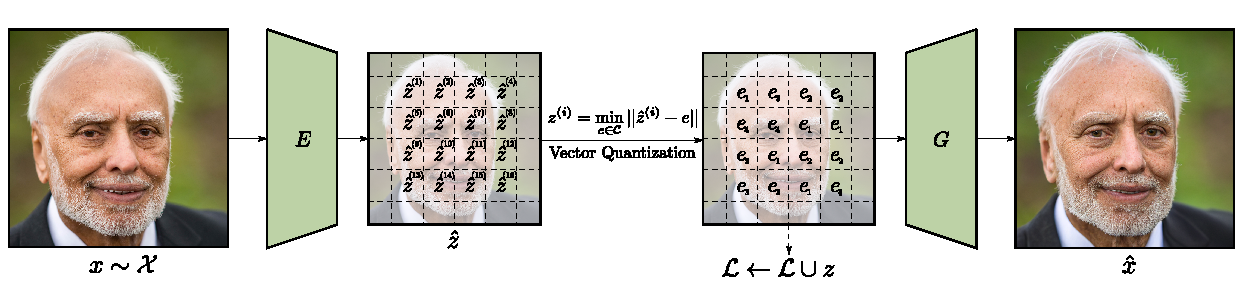
\includegraphics[width=\textwidth]{figures/vq.pdf}
    \caption{
        Visualisation of a vector-quantization image model. An encoder model
        first extracts continuous embeddings from the source image. Vector
        quantization is then used to map each continuous embedding to the
        closest entry in the codebook. A decoder model takes the discretized
        embeddings and attempts to reconstruct the original image. We can
        produce a dataset of latent embeddings from a source image dataset 
        by sampling $\image \sim \imageDataset$ and appending the resulting
        discretized embeddings $\latent$ to a dataset $\latentDataset$.
    }
\end{figure}

Later approaches extended \gls{vqvae} to multiple distinct codebooks in
\acrshort{vqvae}-2~\cite{razavi2019generating}. Though theoretically it can be
extended to any number of codebooks, they performed experiments on a two-level
and three-level model, applying the latter to $1024 \times 1024$ images. They
then sampled the resulting combined discrete codes use
PixelSnail~\cite{chen2017snail}, each code conditioned on all previous levels in
the hierarchy. Though faster to sample than applying a generative directly to
pixels, at such a resolution and with multiple levels to sample, sampling times
were still slow.

Aside from sampling autoregressively, a reason for the slow sampling speed was
the large spatial resolution of the discrete codes. Albeit smaller than the
original signal, \gls{vqvae} is limited in how much it can compress the signal
via a simple reconstruction objective before it loses too much perceptual
quality due to the rate-distortion trade-off. For example, the original
\gls{vqvae} only has a downsampling rate of
$\vqganDownsample=4$~\cite{oord2017vqvae} and \gls{vqvae}-2 has a rate of
top-level rate of $\vqganDownsample=32$ but requires a total of three discrete
latent codes in order to achieve this~\cite{razavi2019generating}. By
introducing perceptual and adversarial loss terms,
\gls{vqgan}~\cite{esser2021taming} is able to achieve compression rates of
$\vqganDownsample=16 \sim 32$ with only a single discrete latent representation
whilst retaining high quality reconstructions~\cite{esser2021taming}. The
greater weighting on perceptual and adversarial loss does mean, however, that
\gls{vqgan} does sometimes edit its reconstructions, rather than attempt to
preserve all details perfectly like when using a simple reconstruction loss
alone. Later, improvements such as differential data
augmentation~\cite{bondtaylor2021unleashing}, codebook improvements, and a
transformer-based architecture~\cite{yu2021vqgan} improved reconstruction
quality further.

Originally designed for audio compression~\cite{zeghidour2021soundstream},
Residual \gls{vq} proposes the use of multiple codebooks to recursively quantize
and refine the residual of an input signal. This produces multiple discrete
representations, which can later be reconstructed by the decoder to decompress
the waveform. Additionally, individual codebooks can be dropped out, allowing
for variable bit-rates~\cite{zeghidour2021soundstream}. Concurrently to this
work, \citet{lee2022rqvae} used residual \gls{vq} to represent images with a
compression ratio of $\vqganDownsample=32$ and then trained a transformer model
to autoregressively predict the stack of discrete tokens at a given spatial
location, allowing for fast sampling despite actually having multiple levels of
discrete latent representations\cite{lee2022rqvae}.

\begin{table}[ht]
    \centering
    \begin{tabular}{|c|c|c|c|c|c|}
        \hline
        \textbf{Model} & \textbf{Input Size} & \textbf{Latent Shape} & \textbf{Codebook Size} & \textbf{FID/val} & \textbf{FID/train} \\
        \hline
        VQ-VAE & $128 \times 128$ & $32 \times 32$ & $512$ & -- & -- \\
        \hline
        VQ-VAE-2 & $256 \times 256$ & $64 \times 64$ \& $32 \times 32$ & $512$ & --& $\sim 10$ \\
                 & $1024 \times 1024$ & $128 \times 128$ \& $64 \times 64$ \& $32 \times 32$ & $512$ & -- & -- \\
        \hline
        DALLE & $256 \times 256$ & $32 \times 32$ & $8192$ & $32.01$ & $33.88$ \\
        \hline
        VQ-GAN & $256 \times 256$ & $16 \times 16$ & $1024$ & $7.94$ & $10.54$ \\
        & $256 \times 256$ & $16 \times 16$ & $16384$ & $4.98$ & $7.41$ \\
        & $256 \times 256$ & $32 \times 32$ & $8192$ & $1.49$ & $3.24$ \\
        & $256 \times 256$ & $64 \times 64$ \& $32 \times 32$ & $8192$ & $1.45$ & $2.78$ \\
        \hline
        RVQ-VAE & $256 \times 256$ & $8 \times 8 \times 2$ & $16384$ & -- & $10.77$ \\
        & $256 \times 256$ & $8 \times 8 \times 4$ & $16384$ & -- & $3.20$ \\
        & $256 \times 256$ & $8 \times 8 \times 8$ & $16384$ & -- & $2.69$ \\
        & $256 \times 256$ & $8 \times 8 \times 16$ & $16384$ & -- & $1.83$ \\
        \hline
    \end{tabular}
    \caption[Table]{Summary of various \acrfull{vq} methods.}
\end{table}

A typical strategy for selecting which codebook vector $e_i$ to map to a
particular input is to compute the Euclidean distance between a given continuous
input and the codebook centroid, and then pick the
$\arg\min$~\cite{oord2017vqvae}. This is denoted the $k$-means strategy. This
strategy does result in a phenomena known as codebook collapse, where certain
codebook vectors never get used, harming the downstream reconstruction quality.
An alternative method is to use the Gumbel-Softmax~\cite{jang2016gumbel} to
select codebook vectors, which typically increases codebook utilisation but
often leads to worse reconstruction quality~\cite{bondtaylor2021unleashing}.

The issue of codebook collapse is quite significant and there have been a number
of attempts to remediate it. \cite{yu2021vqgan} found that a lower codeword
dimension and codeword normalization improved utilisation.
\cite{zeghidour2021soundstream} proposed setting a threshold for ``stale'' codes,
and reinitialisating them to a random vector from the current batch when they
fall below this threshold. \cite{lee2022rqvae} proposed the sharing of a single
codebook across many quantizers and additionally stochastically sampled the
codes as a function of their distance to the centroid, rather than always taking
the $\arg\min$.

All these previous approaches use \gls{vq} models to enhance existing
\gls{ar} models, primarily to improve their sampling speed by reducing the
spatial dimension we are operating over. Few work directly addresses the
discrete prior model itself. Discrete diffusion
models~\cite{austin2021structured} are \gls{nar} approach to generate discrete
data. This was applied to \gls{vqgan} latents in
\citet{bondtaylor2021unleashing}, allowing for fast sampling, flexible
inpainting, and high fidelity outputs.

\subsection{Step-unrolled Denoising Autoencoder}
\label{subsec:sundae}
One recent \gls{nar} model is \gls{sundae}~\cite{savinov2022stepunrolled} which
was evaluated on three language modelling tasks: unconditional text-generation,
inpainting of Python code, and machine translation -- setting a new
state-of-the-art among \gls{nar} models for the machine translation
task~\cite{savinov2022stepunrolled}. It also demonstrates exceptionally fast
sampling, producing high quality samples in as few as 10 steps.

\gls{sundae} is trained using a denoising objective, akin to the
BERT denoising objective~\cite{wang2019bert} but with multiple denoising steps.
Given a uniform prior $p_0$ over some space $\latentSpace = \{1, \dots,
\vqganNbLatents\}^N$ where $N$ is the size of the space and $v$ is the
vocabulary size, consider the Markov process $\latent_t \sim \sundae(\cdot \vert
\latent_{t-1})$ where $\sundae$ is a neural network parameterised by
$\sundaeParameters$, then $\{\latent_t\}_t$ forms a Markov chain. This gives a
$t$-step transition function: \begin{equation}\label{eq:markov} p_t(\latent_t
    \vert \latent_0) = \sum\limits_{\latent_1, \dots, \latent_{t-1} \in
    \latentSpace} \prod\limits^t_{s=1} \sundae(\latent_s | \latent_{s-1})
\end{equation}\cite{savinov2022stepunrolled} and, given a constant number of
steps $\markovSteps$, our model distribution
$p_\markovSteps(\latent_\markovSteps \vert \latent_0)p_0(\latent_0)$ -- which is
clearly intractable.

Instead, they propose an \textit{unrolled denoising} training method that uses a
far lower $\markovSteps$ than is used for
sampling~\cite{savinov2022stepunrolled}. To compensate, they unroll the Markov
chain to start from corrupted data produced by a \textit{corruption
distribution} $\latent' \sim \corruptionDistribution(\cdot \vert \latent)$
rather than from the prior $p_0$ so the model encounters samples more akin to
those seen during the full unroll at sample time~\cite{savinov2022stepunrolled}.
Typically, $\markovSteps = 2$ during training, as a single step would be similar
to the training strategy of BERT~\cite{devlin2019bert} but would lead to worse
performance as seen in earlier work using BERT as a random field language
model~\cite{wang2019bert}.

The training objective of \gls{sundae} is simply the average of all reconstruction
losses $\lossFunction{1:T} = \frac{1}{T} \left(\lossFunction{1} + \dots +
\lossFunction{T} \right)$ of the chain after $t$ steps, which is shown to form
an upper bound on the actual negative
log-likelihood~\cite{savinov2022stepunrolled}. Taking more steps $\markovSteps$
leads to a minor improvement in performance, but considerably slows down
training time~\cite{savinov2022stepunrolled} and increases memory usage.

One advantage of this approach is that sampling starts from random tokens,
rather than a dedicated ``masking''
token~\cite{bondtaylor2021unleashing,austin2021structured}. Unmasking approaches
means that $\markovSteps \leq N$ as at minimum, one token is unmasked per step.
Additionally, it allows the model to be able to ``change its mind'' about
previously predicted positions during sampling, allowing it to make fine-grained
adjustments or fix accumulated errors.

\subsection{Hourglass Transformers}
\label{subsec:hourglass}

Vanilla transformers incur a hefty memory and time complexity of $O(L^2)$ for
each block~\cite{vaswani2017attention}. This is largely due to the multi-head
self-attention mechanism, as each input position must attend to every other.
Most research into efficient transformers focuses on improving the efficiency of
these attention mechanism, such as through sparse attention patterns or
approximations of attention.

Recent work however, is now focusing on making the overall architecture more
efficient. Funnel-Transformer~\cite{dai2020funneltransformer} progressively
downsamples the input sequence and hence reduces the computational cost of the
model. The saved \glspl{flop} can then be reassigned to create deeper or wider models
and thus outperform vanilla transformers given the same computational
budget~\cite{dai2020funneltransformer}. However, the final layer does not
operate at the same granularity as the input, making it unusable for tasks that
require this such as per-token classification or generative tasks. Hourglass
transformers~\cite{nawrot2021hierarchical} include both up- and down-sampling
mechanisms, resulting in a computational saving whilst still being
general-purpose models.


\section{Methodology}\label{sec:method}
% TODO: figures for the following:
% - Latent dataset generation
% - High level overview of hourglass
% - 2d aware modifications: 2d rotary embeddings and downsampling in two
%   directions (showing failings of previous)
% - show training procedure (original z, corruption function, unrolled
%   training). show samples at each step? or save for eval
% - show sampling procedure (random z_0, unrolled steps, show samples, binary
%   mask)
% - show inpainting procedure (modification to binary mask)
% - show some nice samples!

\subsection{Latent Dataset Generation}
We use the standard two-stage scheme for vector-quantized image
modelling~\cite{oord2018neural,razavi2019generating,esser2021taming,bondtaylor2021unleashing} using
VQ-GAN~\cite{esser2021taming} as our feature extractor. Where such models are
available, we use pretrained VQ-GANs for our experiments. For higher resolution
experiments (for example, FFHQ-1024~\cite{karras2019stylebased}), pretrained
models are not available and so training our own VQ-GAN was necessary (see
\S\ref{sec:megagan}).

The second stage is to learn a discrete prior model over these latent variables.
To enable this, we must first build a latent dataset using our trained VQ-GAN.
Formally, given a dataset of images $\imageDataset$, a VQ-GAN encoder
$\vqganEncoder$ with downsample factor $\vqganDownsample$, and vector-quantization codebook $\vqganCodebook$ trained on $\imageDataset,$ we define
our latent dataset $\latentDataset$ as:
\begin{equation}
    \latentDataset = \{\vqganCodebook(\vqganEncoder(\image)) \mid \image \in \imageDataset \}
\end{equation}
where $\image \in \real{3 \times H \times W}$ is a single element of the image
dataset and $\latent = \vqganCodebook(\vqganEncoder(\image)) \in \{1, \dots,
|\vqganCodebook|\}^{h \times w}$ is the corresponding discrete latent
representation. In other words, each $\vqganDownsample \times \vqganDownsample$
pixels in $\image$ is mapped to a single discrete value from $1$ to
$|\vqganCodebook|$ (which in turn, corresponds to a vector $\codebookVector \in
\vqganCodebook$),
resulting in a latent representation of shape $\frac{H}{f} \times \frac{W}{f} =
h \times w$.

We then use $\latentDataset$ to train a discrete prior over the latents. Coupled
with the VQ-GAN decoder $\vqganDecoder$, we obtain a powerful generative model. 

\subsection{2D-Aware Hourglass Transformer}
Inspired by successes in hierarchical transformers for generative language
modelling~\cite{nawrot2021hierarchical}, we modify their architecture for use
with discrete latent representations of image data. We will later use this
architecture as the discrete prior over the VQ-GAN latents. 

Hourglass transformers have been seen to efficiently handle long-sequences,
outperform existing models using the same computational budget, and meet the
same performance as existing models more efficiently by using an explicit
hierarchical structure~\cite{nawrot2021hierarchical}. The same benefits should
also apply to vector-quantized image modelling.

Our modifications are 2D-aware downsampling, axial rotary embeddings, and
removal of causal modelling constraints.

\subsubsection*{2D-Aware Downsampling}
foobar

\subsubsection*{Axial Rotary Embeddings}
foobar

\subsubsection*{Removal of Causal Constraints}
foobar

\subsection{Non-Autoregressive Generator Training}

\subsection{Generating High-Resolution Images}

\subsection{Arbitrary Pattern Inpainting}

\subsection{Training a megapixel VQ-GAN}
\label{sec:megagan}


\section{Evaluation}\label{sec:evaluation}
\subsection{Unconditional Image Generation}

We evaluate our method on the task of unconditional image generation on datasets
FFHQ256, FFHQ1024, CelebA, LSUN Churches, and LSUN Bedrooms. For LSUN we use
pretrained \gls{vqgan} checkpoints provided by~\cite{bondtaylor2021unleashing},
and for all other unconditional experiments we use checkpoints from the original
work~\cite{esser2021taming}. We evaluate in terms of raw perceptual quality and
coverage, as well as how these metrics are affected by the various
hyperparameters of our model and parameters of the sampling process -- the
latter of which we found to be highly configurable.

\subsection{Conditional Image Generation}

Another critical component of an ideal generative model is the ability to
control its generation. We explore class-conditioned image generation of
ImageNet at $256 \times 256$ resolution, using the pretrained ImageNet
\gls{vqgan} checkpoints provided by the original work~\cite{esser2021taming}. To
introduce class information to the model, we add an additional embedding layer
(one embedding for each of the 1000 classes) and add this to all input token
embeddings, as done in Image Transformer~\cite{parmar2018image}. We again,
perform our evaluation using metrics of perceptual quality and distribution
coverage.

\subsection{Arbitrary Image Inpainting}

As outlined earlier, \acrlong{nar} generative models have a number of advantages
on inpainting tasks, including supporting arbitrary masks and being able to use
the full context available to them. We provide a number of examples of
inpainting on FFHQ1024 and ImageNet, showcasing different patterns and different
results given the same starting image. As our method utilises a vector quantized
image model, it is incapable of doing fine-grained inpainting at a pixel level.
Nonetheless, the results show consistently good inpainting results when
operating at a \gls{vq} latent level.


\section{Conclusion}\label{sec:conclusion}
In this work, we proposed using denoising autoencoders for the
non-autoregressive prediction of VQ latents. This enables fast sampling
times and flexible inpainting. In addition, we made changes to the hourglass
transformer architecture to make it more suited for two-dimensional signals.
Additionally, we demonstrate the scalability of our approach by training a
VQ-GAN at extremely high resolutions and training our model on the resulting
latent dataset. Ultimately, this allows for the sampling of high quality and
diverse $1024 \times 1024$ images in mere seconds. Further work is required to
improve sampling time further -- closing the gap with single-step methods like
GANs -- and to improve the reconstruction quality of VQ-GAN when operating at
high downsampling factors.


\bibliographystyle{iclr2022_conference}
{\small \bibliography{references}}

\end{document}
